\begin{figure}[H]
	\centering
	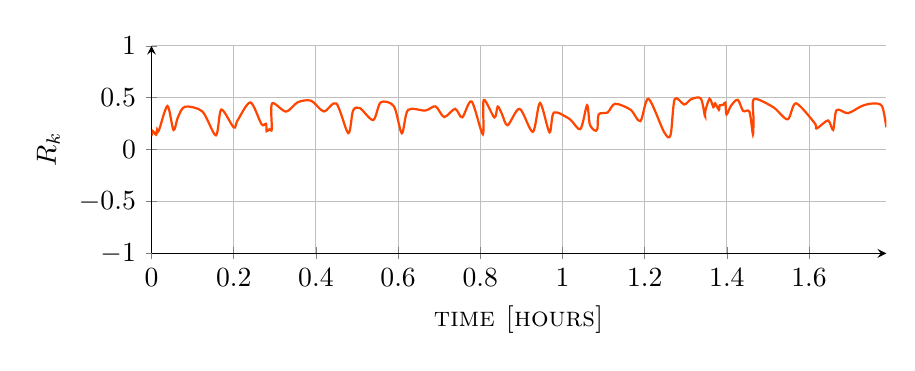
\begin{tikzpicture}
		\begin{axis}[xlabel=\textsc{time [hours]}, ylabel=\textsc{$R_k$}, axis lines=left, grid=major, width=0.9\linewidth, height=12em, ymax=1, ymin=-1]
			\addplot +[mark=none, OrangeRed, thick, smooth] table {
				0.0 0.13135369747917117
				0.0025855555555555554 0.17978227963505983
				0.011065 0.1433706880737134
				0.013418055555555556 0.19059945822298427
				0.017869444444444445 0.1835153962042667
				0.03875805555555555 0.4202933378943818
				0.05345055555555556 0.1889325520806588
				0.06443777777777777 0.31311058973677475
				0.08145416666666667 0.4133930881661661
				0.12378444444444445 0.3669547958847006
				0.15660416666666666 0.13736965312050634
				0.16978138888888888 0.38611082569702654
				0.2001813888888889 0.21295949563893907
				0.20897666666666667 0.2778809466898707
				0.24047916666666666 0.4544524888262656
				0.2677836111111111 0.24383016391240805
				0.27866 0.2488432276112016
				0.27997305555555557 0.17739668799676617
				0.28716250000000004 0.19663401394502
				0.2926694444444444 0.197838982154629
				0.29330999999999996 0.44512835960341024
				0.3273313888888889 0.36618504872674407
				0.3559847222222222 0.4566089407746047
				0.38857138888888887 0.47060581784904165
				0.41923750000000004 0.3675125821824269
				0.44963583333333335 0.4448459674526829
				0.4787425 0.15837773572161426
				0.4904219444444444 0.3760678380869933
				0.5072680555555555 0.39876745490708554
				0.5393652777777778 0.2848333878185541
				0.5578175 0.45573743056753074
				0.5898619444444445 0.41718393823247857
				0.6091241666666667 0.15702276668836215
				0.6241308333333334 0.38185868928710953
				0.6661866666666666 0.3760794206383165
				0.691013611111111 0.4163915799147428
				0.7121916666666667 0.3135146433415765
				0.7386305555555556 0.3930558510204319
				0.7559472222222222 0.31076940881467824
				0.7788469444444445 0.4641318740787899
				0.8062124999999999 0.14731025238025144
				0.8084169444444445 0.4775649272990927
				0.8342591666666667 0.30928714693435644
				0.8423063888888889 0.4144346955585863
				0.8524380555555555 0.3450651726569078
				0.8665238888888889 0.23489365476101703
				0.8956927777777778 0.3928009008824002
				0.9277994444444444 0.1708045609796094
				0.9453472222222222 0.4488435959844424
				0.9684547222222222 0.16619532461045536
				0.9790966666666667 0.3567234468093689
				1.0172505555555555 0.29484504051138977
				1.043455 0.19719231216543037
				1.0597436111111112 0.4265752170560484
				1.0661752777777778 0.24736387237742072
				1.0772247222222222 0.18623329894253718
				1.0848566666666666 0.19889108753805865
				1.088175 0.33998726409747154
				1.1096827777777778 0.3576138154578811
				1.1280069444444445 0.44145864391484957
				1.1654772222222223 0.3844213178737763
				1.1894377777777776 0.2743321383286894
				1.2092597222222223 0.48955161528378266
				1.2472547222222223 0.16860818228690932
				1.2628700000000002 0.13949046133460127
				1.2730925 0.48651846609553856
				1.2961861111111113 0.4342773809966667
				1.3129688888888889 0.48520954886839207
				1.336426388888889 0.4930517092327974
				1.3466094444444443 0.3210927043016705
				1.3472230555555555 0.36879317618542606
				1.357823888888889 0.4905149879403897
				1.3671708333333332 0.4093075816319852
				1.3712952777777776 0.44611682445826717
				1.3805030555555555 0.38241538947618475
				1.3823174999999999 0.4263812520825596
				1.3907119444444445 0.42999655365252887
				1.3962883333333334 0.45224276816124975
				1.3991397222222224 0.33869879244799456
				1.410311388888889 0.4240680585359524
				1.4263894444444445 0.4799486385900556
				1.4395727777777778 0.3718745708563724
				1.4547747222222223 0.3651755368069844
				1.4633144444444444 0.14737214668233004
				1.4648019444444444 0.2935961842077465
				1.4659758333333333 0.48628746128484934
				1.5129652777777778 0.4081586994466556
				1.5477008333333333 0.2916215600448714
				1.5681469444444445 0.4454973343273979
				1.6138030555555556 0.25359413702740863
				1.6184880555555554 0.2029602655554598
				1.6460261111111112 0.2809671161547638
				1.658562222222222 0.1899507640277969
				1.666983611111111 0.3808328309437742
				1.694725 0.3513901811142677
				1.7280508333333333 0.41954360389996287
				1.7539847222222222 0.4436484824239076
				1.7773955555555554 0.4190367076093213
				1.7877955555555556 0.21566842715213244
			};
		\end{axis}
	\end{tikzpicture}
	\caption{Hyper-parameters optimization plot for the category classifier based on extra-trees.}
	\label{fig:optimization_category_extra_trees}
\end{figure}
\begin{table}[H]
	\centering
	\begin{tabular}{ll}
		\toprule
		\textsc{hyper-parameter} & \textsc{value}\\
		\midrule
		\verb|criterion| & entropy\\
		\verb|max_depth| & 20\\
		\verb|min_samples_leaf| & 3\\
		\verb|min_samples_split| & 37\\
		\verb|n_estimators| & 88\\
		\bottomrule
	\end{tabular}
	\caption{Optimal hyper-parameters for the category classifier based on extra-trees.}
	\label{tab:hyperparameters_category_extra_trees}
\end{table}
\begin{table}[H]
	\centering
	\begin{tabular}{lrrrr}
		\toprule
		\textsc{statistic} & \textsc{training set} & \textsc{dev set} & \textsc{kts} & \textsc{uts}\\
		\midrule
		samples & 955872 & 119484 & 119485 & 30144\\
		accuracy [$\%$] & 85.085 & 85.033 & 85.015 & 37.646\\
		balanced accuracy [$\%$] & 80.692 & 80.216 & 80.373 & 38.510\\
		precision [$\%$] & 62.558 & 62.265 & 62.413 & 33.339\\
		recall [$\%$] & 80.692 & 80.216 & 80.373 & 38.510\\
		Cohen’s kappa [$\%$] & 42.760 & 42.372 & 42.547 & 1.694\\
		F-score [$\%$] & 62.138 & 61.837 & 61.866 & 33.949\\
		Jaccard score [$\%$] & 51.661 & 51.322 & 51.552 & 21.426\\
		Hamming loss & 0.149 & 0.150 & 0.150 & 0.624\\
		zero-one loss & 0.149 & 0.150 & 0.150 & 0.624\\
		$R_k$ & 0.491 & 0.487 & 0.489 & 0.017\\
		\bottomrule
	\end{tabular}
	\caption{Classification statistics for the category classifier based on extra-trees.}
	\label{tab:classification_category_extra_trees}
\end{table}
\begin{table}[H]
	\centering
	\begin{tabular}{ll|lll}
	\setlength{\tabcolsep}{2pt}
		 & & \multicolumn{3}{c}{\textsc{inferred}}\\
		 & & \textsc{browser} & \textsc{crawler} & \textsc{dos}\\
		\midrule
		\multirow{3}{*}{\rotatebox{90}{\textsc{target}}} & \textsc{browser} & 5225 & 1496 & 667\\
		 & \textsc{crawler} & 126 & 1954 & 235\\
		 & \textsc{dos} & 1439 & 13942 & 94401\\
	\end{tabular}
	\caption{Confusion matrix for the category classifier based on extra-trees on the KTS.}
	\label{tab:confusion_category_extra_trees}
\end{table}
\begin{figure}[H]
	\centering
	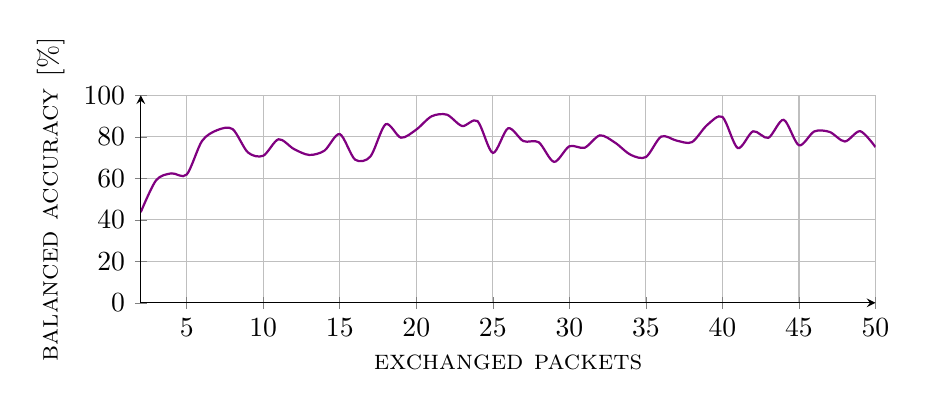
\begin{tikzpicture}
		\begin{axis}[xlabel=\textsc{exchanged packets}, ylabel=\textsc{balanced accuracy [$\%$]}, axis lines=left, grid=major, width=0.9\linewidth, height=12em, ymax=100, ymin=0]
			\addplot +[mark=none, Purple, thick, smooth] table {
				2.0 43.691222570532915
				3.0 59.030648610121176
				4.0 62.37431322090375
				5.0 61.8032169706335
				6.0 77.96059573722181
				7.0 83.21906305576192
				8.0 83.71202582905025
				9.0 72.4771413867778
				10.0 70.86167891470922
				11.0 78.81730045570406
				12.0 74.13348083245074
				13.0 71.2446842703852
				14.0 73.32694532252525
				15.0 81.31408277755185
				16.0 69.00997448387845
				17.0 70.47534074132659
				18.0 86.05512055875252
				19.0 79.5663293873137
				20.0 83.46822475085528
				21.0 89.87217188576273
				22.0 90.64844948459519
				23.0 85.18812930577636
				24.0 87.56313131313132
				25.0 72.2152976022945
				26.0 84.09961685823754
				27.0 77.91341900147461
				28.0 77.34703866862456
				29.0 67.89813486370159
				30.0 75.43031705435797
				31.0 74.73777348777348
				32.0 80.69345941686366
				33.0 77.0947105632704
				34.0 71.32366356504288
				35.0 70.2337345194488
				36.0 80.10717128563243
				37.0 78.16370992841581
				38.0 77.39898989898991
				39.0 85.6612952265126
				40.0 89.56062670299727
				41.0 74.57808323787705
				42.0 82.63428991905813
				43.0 79.48717948717949
				44.0 88.17393342709798
				45.0 75.89490968801314
				46.0 82.57142857142856
				47.0 82.33704829449509
				48.0 77.73671393783125
				49.0 82.6917826917827
				50.0 75.0278706800446
			};
		\end{axis}
	\end{tikzpicture}
	\caption{Balanced accuracy vs. exchange packets plot for the category classifier based on extra-trees on the KTS.}
	\label{fig:packets_category_extra_trees}
\end{figure}
\begin{table}[H]
	\centering
	\begin{subtable}{.45\linewidth}
		\centering
	\begin{tabular}{ll}
		\toprule
		\textsc{inferred class} & \textsc{samples}\\
		\midrule
		browser & 2570\\
		crawler & 1242\\
		dos & 2722\\
		\bottomrule
	\end{tabular}
	\caption{Classification of \textsc{firefox-68.0}.}
	\end{subtable}
	\begin{subtable}{.45\linewidth}
		\centering
	\begin{tabular}{ll}
		\toprule
		\textsc{inferred class} & \textsc{samples}\\
		\midrule
		browser & 837\\
		crawler & 1809\\
		dos & 1019\\
		\bottomrule
	\end{tabular}
	\caption{Classification of \textsc{grabsite-2.1.16}.}
	\end{subtable}
	\begin{subtable}{.45\linewidth}
		\centering
	\begin{tabular}{ll}
		\toprule
		\textsc{inferred class} & \textsc{samples}\\
		\midrule
		browser & 5237\\
		crawler & 1046\\
		dos & 2667\\
		\bottomrule
	\end{tabular}
	\caption{Classification of \textsc{opera-62.0.3331.66}.}
	\end{subtable}
	\begin{subtable}{.45\linewidth}
		\centering
	\begin{tabular}{ll}
		\toprule
		\textsc{inferred class} & \textsc{samples}\\
		\midrule
		browser & 5077\\
		crawler & 4186\\
		dos & 1732\\
		\bottomrule
	\end{tabular}
	\caption{Classification of \textsc{slowhttptest-1.6}.}
	\end{subtable}
	\caption{Classification of unknown tools for the category classifier based on extra-trees.}
	\label{tab:unknown_category_extra_trees}
\end{table}
